\documentclass[a4paper,class=article,border=10pt,tikz]{standalone}

%mypackages
\usepackage{pythontex}
\usepackage{pgfplots}
\usepackage{amsmath}
\usepackage{titlesec}
\usepackage{tikz}
\usetikzlibrary{shapes.geometric}
\usetikzlibrary{positioning}
\usetikzlibrary{snakes,calc,positioning,patterns,angles,quotes,decorations.pathmorphing,decorations.markings}
% \titleformat{<command>}[<shape>]{<format>}{<label>}{<sep>}{<before-code>}[<after-code>]
%\titleformat{\section}{\normalfont\Large\bfseries}{\thesection.}{10pt}{}
% \titlespacing{<command>}{<left>}{<before-sep>}{<after-sep>}
%\titlespacing{\section}{0pt}{14pt}{7pt}

%\titleformat{\subsection}{\normalfont\itshape}{\thesubsection.}{10pt}{}
%\titlespacing{\subsection}{0pt}{12pt}{6pt}
% set font encoding for PDFLaTeX, XeLaTeX, or LuaTeX
\usepackage{ifxetex,ifluatex}
\if\ifxetex T\else\ifluatex T\else F\fi\fi T%
  \usepackage{fontspec}
\else
  \usepackage[T1]{fontenc}
  \usepackage[utf8]{inputenc}
  \usepackage{lmodern}
\fi

\usepackage{hyperref}


\title{Title of Document}
\author{Name of Author}

% Enable SageTeX to run SageMath code right inside this LaTeX file.
% http://doc.sagemath.org/html/en/tutorial/sagetex.html
% \usepackage{sagetex}

% Enable PythonTeX to run Python – https://ctan.org/pkg/pythontex
% \usepackage{pythontex}

\begin{document}

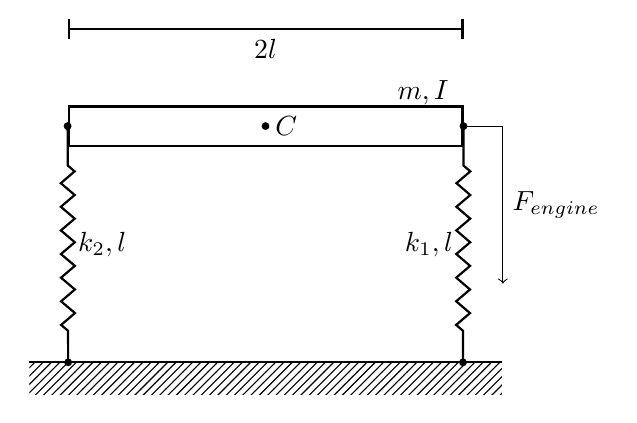
\begin{tikzpicture}
 \coordinate (origo) at (0,0);

\tikzstyle{spring}=[thick,decorate,decoration={zigzag,pre length=0.4cm,post length=0.4cm,segment length=0.3cm}]

   %draw roof
    %\fill[pattern = north east lines] ($ (origo) + (-3,0) $) rectangle ($ (origo) + (3,0.3) $);
    

    \tikzstyle{ground}=[fill,pattern=north east lines,draw=none,minimum width=5cm,minimum height=0.3cm]
    
        %\node (ground) [ground,anchor=north west,xshift=-2.4cm,yshift=-0.25cm,minimum width=5cm] {};
    

   \node (ground) [ground,anchor=north ,xshift=0cm,yshift=-3cm,minimum width=6cm,minimum height=0.4cm] at (origo)   {};
   \draw[thick] (ground.north west) -- (ground.north east);
   
   \node (M) at (origo) [draw,thick,minimum width=5cm, minimum height=0.5cm]{};
    \node (m1_label) at ($(M) + (2,0.7)$) [below] {$m, I$};

    \draw [spring] (ground.north west) ++ (0.5,0) node (ground_fix_L) {} -- (M.west) node [midway,right] {$k_2, l$};
    \draw [spring] (ground.north east) ++ (-0.5,0) node (ground_fix_R)  {} -- (M.east) node [midway,left] {$ k_1,l$};


    \fill [black] (M.center) circle (0.05) node [right] (c_label) {$C$};

    \fill [black] (ground_fix_L) circle (0.05) ;
    \fill [black] (ground_fix_R) circle (0.05);
    \fill [black] (M.east) circle (0.05) ;
    \fill [black] (M.west) circle (0.05);


    \draw[thick,|-|]  (M.south west) ++ (0cm,1.5cm) --  ([yshift=1.5cm]M.south east)  node[midway, below] {$2l$};
    \draw[thin] (M.east)--++(0.5cm,0) node (force_point){};
    \draw[->](force_point.center)--++(0,-2cm) node[midway,right] {$F_{engine}$};


\end{tikzpicture}
\end{document}
% \draw[<->,line width=1.5pt] (-0.5,0)--(0.5,0) node[midway,above]{$x_{e}(t)$};